% Lecture Template for ME3023 -  Measurements in Mechanical Systems - Tennessee Technological University
% Spring 2020 - Summer 2020 - Fall 2020 - Spring 2021 - Summer 2021 - Fall 2023
% Tristan Hill, May 07, 2020 - June 12, 2020 - July 08, 2020 - Novemeber 02, 2020 - March 28, 2021 - May 25, 2021 - August 21, 2022 - September 02, 2023 - September 09, 2023 - April 07, 2024 

% Fall 2023 - condensing and streamlining lectures by combining topics into a single PDF under the module name
%			  this will simplify file and link management as well as make lectures easier to use in class
%			- added image/ to clean directory and reduce redundancy, specific to module for now  

% Module Name: - Data Acquisition

\documentclass[fleqn]{beamer} % for presentation (has nav buttons at bottom)
\usepackage{../measurements_lectures}

\author{ME3023 - Measurements in Mechanical Systems} 

\newcommand{\MNUM}{9\hspace{2mm}} % module number 
\newcommand{\moduletitle}{Strain Gauges}

\newcommand{\sectionItitle}{Measuring Strain}
\newcommand{\sectionIItitle}{The Wheatstone Bridge}
\newcommand{\sectionIIItitle}{P3 Strain Indicator}

\newcommand{\sectionIsubsectionItitle}{Motivation in Design}
\newcommand{\sectionIsubsectionIItitle}{Stress and Strain}
\newcommand{\sectionIsubsectionIIItitle}{The Strain Gauge}
\newcommand{\sectionIsubsectionIVtitle}{Engineering Applications}

\newcommand{\sectionIIsubsectionItitle}{Resistive Gauges}
\newcommand{\sectionIIsubsectionIItitle}{The Bridge Circuit}
\newcommand{\sectionIIsubsectionIIItitle}{Balancing the Bridge}
\newcommand{\sectionIIsubsectionIVtitle}{Gauge Sensitivity}

\newcommand{\sectionIIIsubsectionItitle}{Units of Microstrain}
\newcommand{\sectionIIIsubsectionIItitle}{Quarter, Half, and Full Configuration}
\newcommand{\sectionIIIsubsectionIIItitle}{Operating the P3}
\newcommand{\sectionIIIsubsectionIVtitle}{Alternative Solutions}

 \newcommand{\btVFill}{\vskip0pt plus 1filll}

% custom box
\newsavebox{\mybox}

\title{Lecture Module - \moduletitle}

\date{Mechanical Engineering\vspc Tennessee Technological University}

\begin{document}

	\lstset{language=MATLAB,basicstyle=\ttfamily\small,showstringspaces=false}

	\frame{\titlepage \center\begin{framed}\Large \textbf{Module \MNUM - \moduletitle}\end{framed} \vspace{5mm}}

	% Module Outline
	\begin{frame} 
		\large \textbf{Module \MNUM - \moduletitle} \vspace{3mm}\\

		\begin{itemize}
			\item Topic 1 - \hyperlink{sectionI}{\sectionItitle} \vspc % section I
			\item Topic 2 - \hyperlink{sectionII}{\sectionIItitle} \vspc % section II
			\item Topic 3 - \hyperlink{sectionIII}{\sectionIIItitle} \vspc % section III
		\end{itemize}

	\end{frame}

	% section I
	\section{\sectionItitle}\label{sectionI}

		% section I Outline
		\begin{frame} 
			\large \textbf{Topic 1 - \sectionItitle} \vspace{3mm}\\

			\begin{itemize}
				\item \hyperlink{sectionIsubsectionI}{\sectionIsubsectionItitle} \vspc %  section I subsection I
				\item \hyperlink{sectionIsubsectionII}{\sectionIsubsectionIItitle} \vspc % section I subsection II
				\item \hyperlink{sectionIsubsectionIII}{\sectionIsubsectionIIItitle} \vspc % section I subsection III
				\item \hyperlink{sectionIsubsectionIV}{\sectionIsubsectionIVtitle} \vspc % section I subsection IV
			\end{itemize}
		\end{frame}
		
		% section I subsection I 
		\subsection{\sectionIsubsectionItitle}\label{sectionIsubsectionI}

			\begin{frame}
				\frametitle{\sectionIsubsectionItitle}

				The design of load-carrying components for machines and structures requires information concerning the {\BL distribution of forces within the particular component}. Proper design of devices such as shafts, pressure vessels, and support structures must consider {\PR load-carrying capacity and allowable deflections}. Mechanics of materials provides a basis for predicting these essential characteristics of a mechanical design, and provides the fundamental understanding of the behavior of load-carrying parts. However, theoretical analysis is often not sufficient, and {\PN experimental measurements} are required to achieve a final design.

				{\tiny Text: Theory and Design of Mechanical Measurements}
		
			\end{frame}

			\begin{frame}
				\frametitle{\sectionIsubsectionItitle}


				\btVFill
			
			\end{frame}


		% section I subsection II
		\subsection{\sectionIsubsectionIItitle}\label{sectionIsubsectionII}

			\begin{frame}
				\frametitle{\sectionIsubsectionIItitle}\small
				\bigskip

				Consider a member under uni-axial loading. The {\RD strain} is defined as the ratio of the change in length to the original length of the  component.  

				\begin{multicols}{2}
				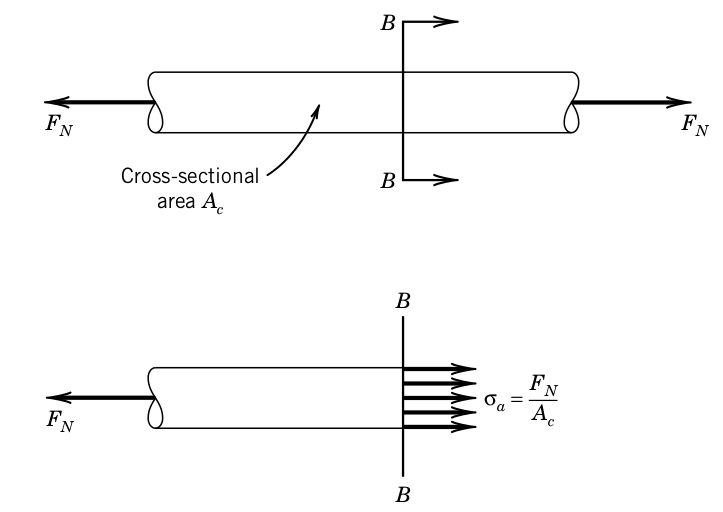
\includegraphics[scale=.25]{images/strain_fig1.png}


				\hspace{15mm}\scalebox{1}{$\sigma_a=\frac{F_N}{A_c}$}\vspace{10mm}\\
				\hspace{15mm}\scalebox{1}{$\epsilon_a=\frac{\delta_L}{L}$}\vspace{10mm} \\
				\hspace{15mm}\scalebox{1}{$\sigma_a=E_m\epsilon_a$}\vspc
				\end{multicols}

				\btVFill
				
			\end{frame}

			\begin{frame}
				\frametitle{\sectionIsubsectionIItitle}\small
				\bigskip

				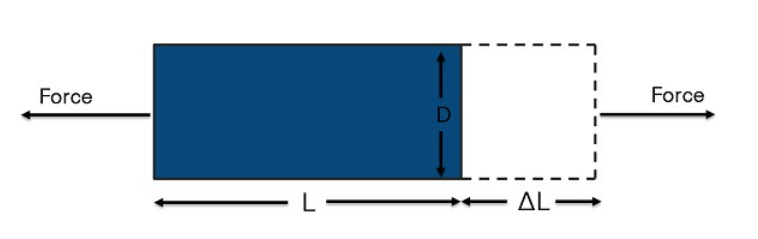
\includegraphics[scale=.20]{images/strain_fig2.png} 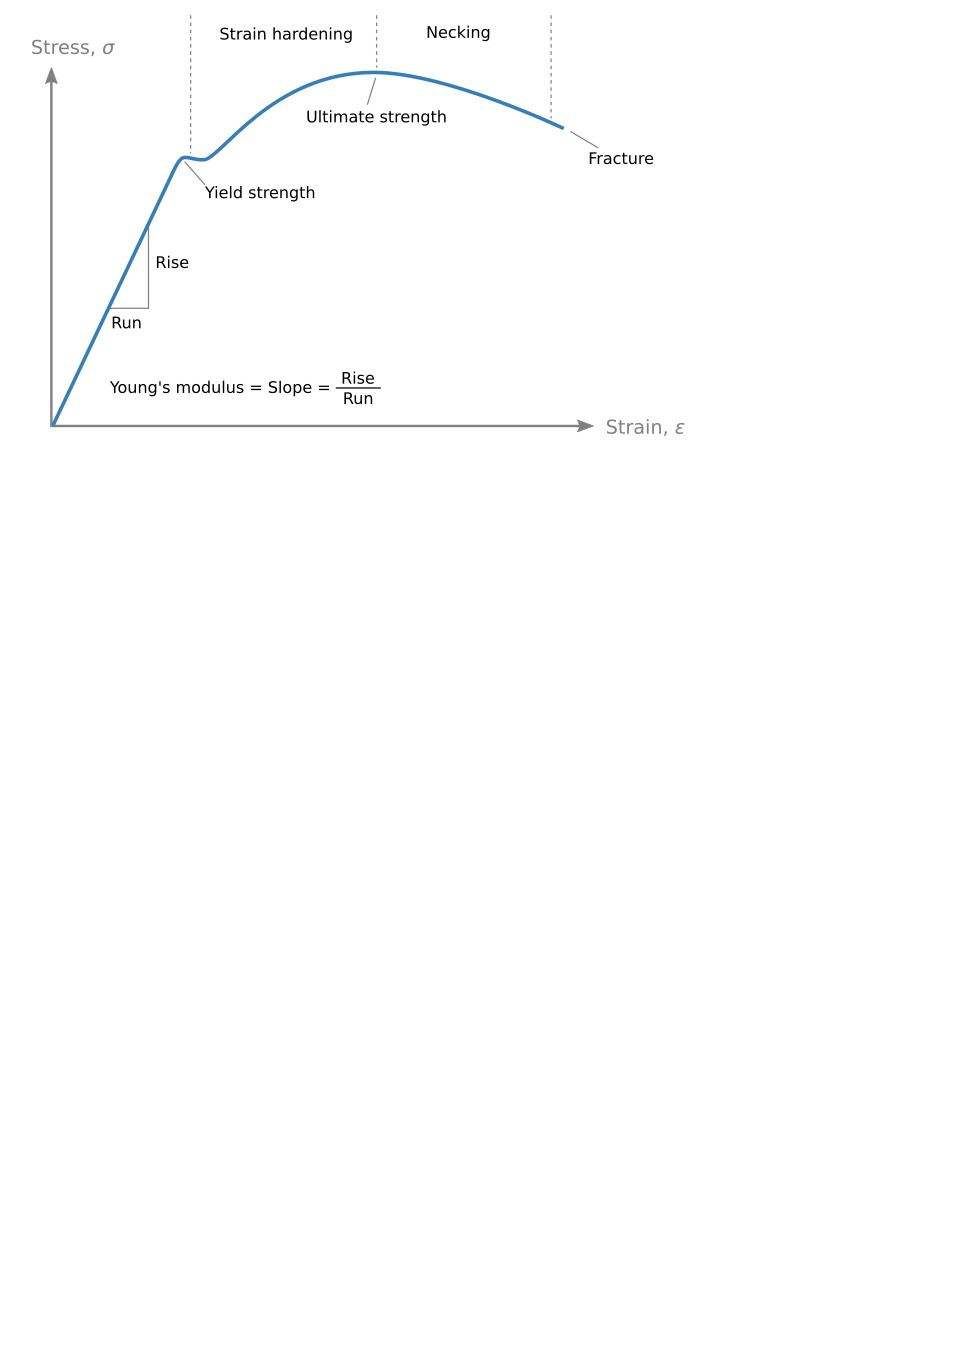
\includegraphics[scale=.5]{images/stress_strain_fig1.png} 
				\btVFill
{\tiny Image: \href{https://commons.wikimedia.org/wiki/File:Stress_strain_ductile.svg}{Wikimedia} }

			\end{frame}

		% section I subsection III
		\subsection{\sectionIsubsectionIIItitle}\label{sectionIsubsectionIII}
			\begin{frame} 
				\frametitle{\sectionIsubsectionIIItitle} \scriptsize

				... the ideal sensor for the measurement of strain would (1) have good spatial resolution, implying
				that the sensor would measure strain at a point; (2) be unaffected by changes in ambient conditions;
				and (3) have a high-frequency response for dynamic (time-resolved) strain measurements. A sensor
				that closely meets these characteristics is the {\BL bonded resistance strain gauge}. \vspc

				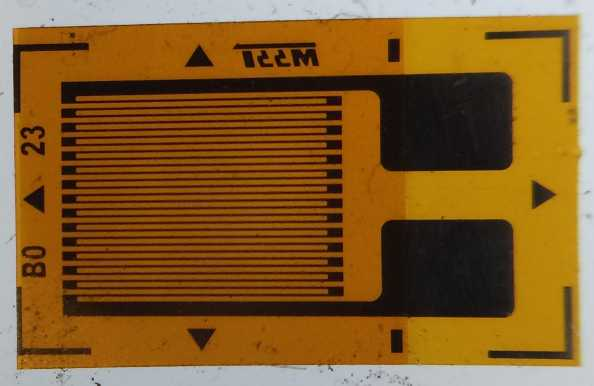
\includegraphics[scale=.20]{images/unmounted_strain_gauge.jpg}\hspccc 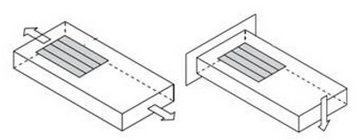
\includegraphics[scale=.4]{images/mounted_gages.png}

				\bigskip
				{\tiny Text: Theory and Design of Mechanical Measurements}

				
			\end{frame}	

			\begin{frame} 
				\frametitle{\sectionIsubsectionIIItitle}

				Strain gauges can be mounted in different ways for different purposes. We will begin with a single gauge mounted in the axial direction. \vspc

				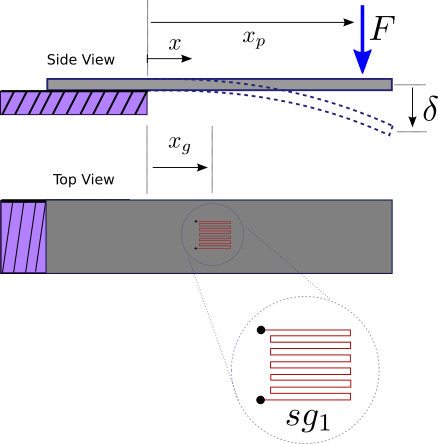
\includegraphics[scale=.4]{images/axial_gaged_beam.png}

				\bigskip
				{\tiny Text: Theory and Design of Mechanical Measurements}

				
			\end{frame}	

		% section I subsection IV
		\subsection{\sectionIsubsectionIVtitle}\label{sectionIsubsectionIV}	

			\begin{frame}
				\frametitle{\sectionIsubsectionIVtitle} \scriptsize
				\bigskip

				\begin{itemize}

				\item Segway back to {\it Motivation in Design} (Slide 1) ... \vspc

				\item Aerospace \vspc

				\item Infrastructure \vspc

				\item Short article on applications \href{https://medium.com/@encardio/strain-gauge-principle-types-features-and-applications-357f6fed86a5}{here}. 

				\end{itemize}
			
				\btVFill
				\tiny{some reference}	

			\end{frame}

			\begin{frame}
				\frametitle{\sectionIsubsectionIVtitle} \scriptsize


			\end{frame}


			\begin{frame}
				\frametitle{\sectionIsubsectionIVtitle} \scriptsize

				\bigskip


				\btVFill

										
			\end{frame}

	
	% Section II
	\section{\sectionIItitle}\label{sectionII}

		% section II Outline
		\begin{frame}
			\large \textbf{Topic 2 - \sectionIItitle} \vspace{3mm}\\

			\begin{itemize}
				\item \hyperlink{sectionIIsubsectionI}{\sectionIIsubsectionItitle} \vspc %  section II subsection I
				\item \hyperlink{sectionIIsubsectionII}{\sectionIIsubsectionIItitle} \vspc % section II subsection II
				\item \hyperlink{sectionIIsubsectionIII}{\sectionIIsubsectionIIItitle} \vspc % section II subsection III
				\item \hyperlink{sectionIIsubsectionIV}{\sectionIIsubsectionIVtitle} \vspc % section II subsection IV
			\end{itemize}

		\end{frame}

		% section II subsection I
		\subsection{\sectionIIsubsectionItitle}\label{sectionIIsubsectionI}

			\begin{frame}[label=sectionIIsubsectionI]
				\frametitle{\sectionIIsubsectionItitle} \scriptsize

				\bigskip	
				The resistive strain gauge, aka {\it metallic gauge}, is bonded to the surface so that is deforms with the specimen. The change in length of the bonded gauge causes a change in resistance which is used as a measure of strain. \vspccc

				\scalebox{1}{$R=\rho_eL/A_c=fn(L, ...)$}

				\begin{multicols}{2}

				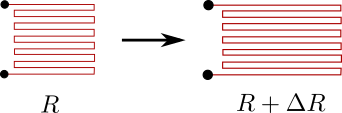
\includegraphics[scale=0.5]{images/stretched_gauge.png}

				This is an exaggerated picture so the change is  very small...

				\end{multicols}

				
				
				\btVFill
				{\tiny Images: T.Hill}
		
			\end{frame}

		    \begin{frame}[label=sectionIIsubsectionI]
				\frametitle{\sectionIIsubsectionItitle} \scriptsize

				The {\PN Gauge Factor} is typically used instead of the physical parameters. \vspcc

				\scalebox{1}{$GF \equiv \frac{\delta R/R}{\delta L/L}=\frac{\delta R/R}{\epsilon_a}$}\vspcc

				This number relates the relative change in resistance to the measured strain. \vspc

				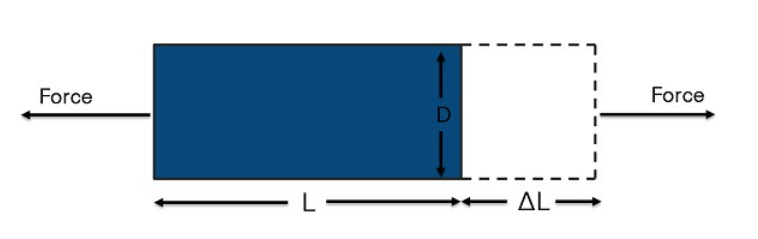
\includegraphics[scale=.25]{images/strain_fig2.png}

				\btVFill

				{\tiny Images: \href{https://www.ni.com/en-us/innovations/white-papers/07/measuring-strain-with-strain-gages.html}{NI}}
					
			\end{frame}	


		% section II subsection II
		\subsection{\sectionIIsubsectionIItitle}\label{sectionIIsubsectionII}

			\begin{frame}
				\frametitle{\sectionIIsubsectionIItitle} \scriptsize
				\bigskip

				\begin{multicols}{2}

				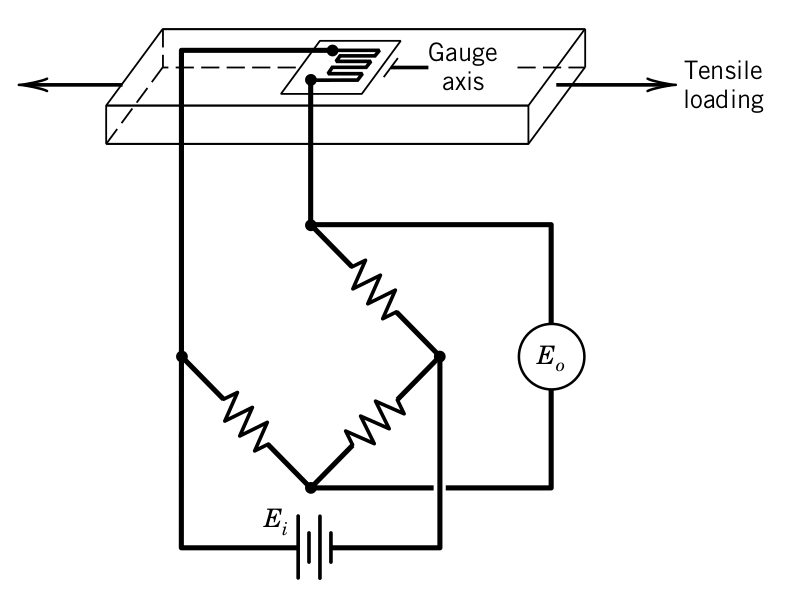
\includegraphics[scale=.25]{images/gauged_beam_bridge.png} \vspace{15mm} 

				A {\PR transducer} converts the sensed information into a detectable signal. The signal might be mechanical, electrical, optical, or may take any other form that can be meaningfully recorded.

				\end{multicols}

				\btVFill
				{\tiny Text. Images: Theory and Design for Mechanical Measurements}

			\end{frame}

			\begin{frame}
				\frametitle{\sectionIIsubsectionIItitle} \scriptsize
	
				\bigskip

				\begin{multicols}{2}

				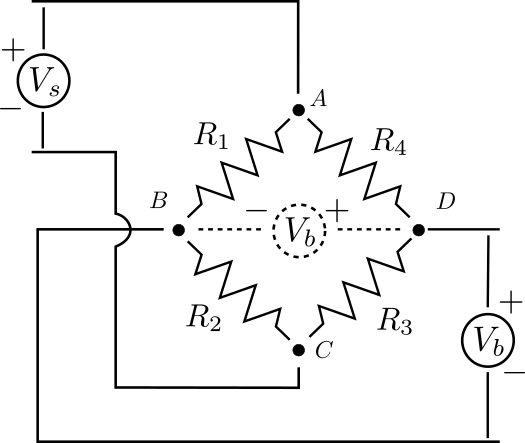
\includegraphics[scale=.35]{images/bridge_circuit.png} \vspace{15mm} 

				How does the bridge circuit work as a transducer? \vspc Use KVL and the voltage divider rule find the relationship between the two voltages. \vspc

				\scalebox{1}{$V_b=\left( \frac{R_3}{R_3+R_4}-\frac{R_2}{R_1+R_2}\right)\times V_s$}

				\end{multicols}
				 
				\btVFill
				{\tiny Images: T.Hill}
				
			\end{frame}

		% section II subsection III
		\subsection{\sectionIIsubsectionIIItitle}\label{sectionIIsubsectionIII}

			\begin{frame}
				\frametitle{\sectionIIsubsectionIIItitle} 

				\bigskip

				If all four resistors are equal the bridge voltage will equal zero and the bridge is said it be {\BL balanced}. 
				One or more resistors in the circuit is replaced by a strain gauge and bridge voltage is used as a measure of change in resistance and therefore strain. \vspc

				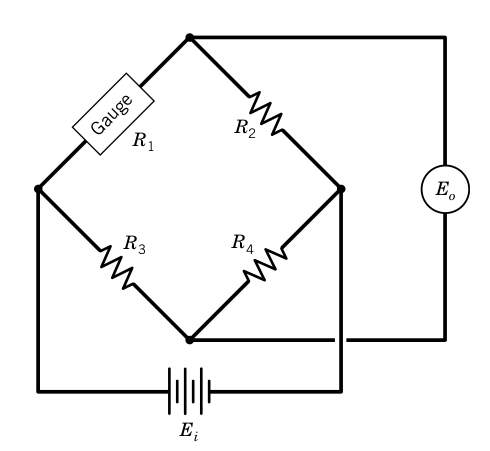
\includegraphics[scale=.2]{images/gauge_in_bridge_quarter.png} 

				This gives a linear {\PR calibration curve} with a convenient {\RD zero offset}. \vspc 
				
				\btVFill
				{\tiny Text. Images: Theory and Design for Mechanical Measurements}

			\end{frame}

			\begin{frame}
				\frametitle{\sectionIIsubsectionIIItitle}

				\bigskip


				\btVFill
			
			\end{frame}

			\begin{frame}
			\frametitle{\sectionIIsubsectionIIItitle}




				\btVFill

			\end{frame}

		% section II subsection IV 
		\subsection{\sectionIIsubsectionIVtitle}\label{sectionIIsubsectionIV}

			\begin{frame}
				\frametitle{\sectionIIsubsectionIVtitle}

				\begin{multicols}{2}

				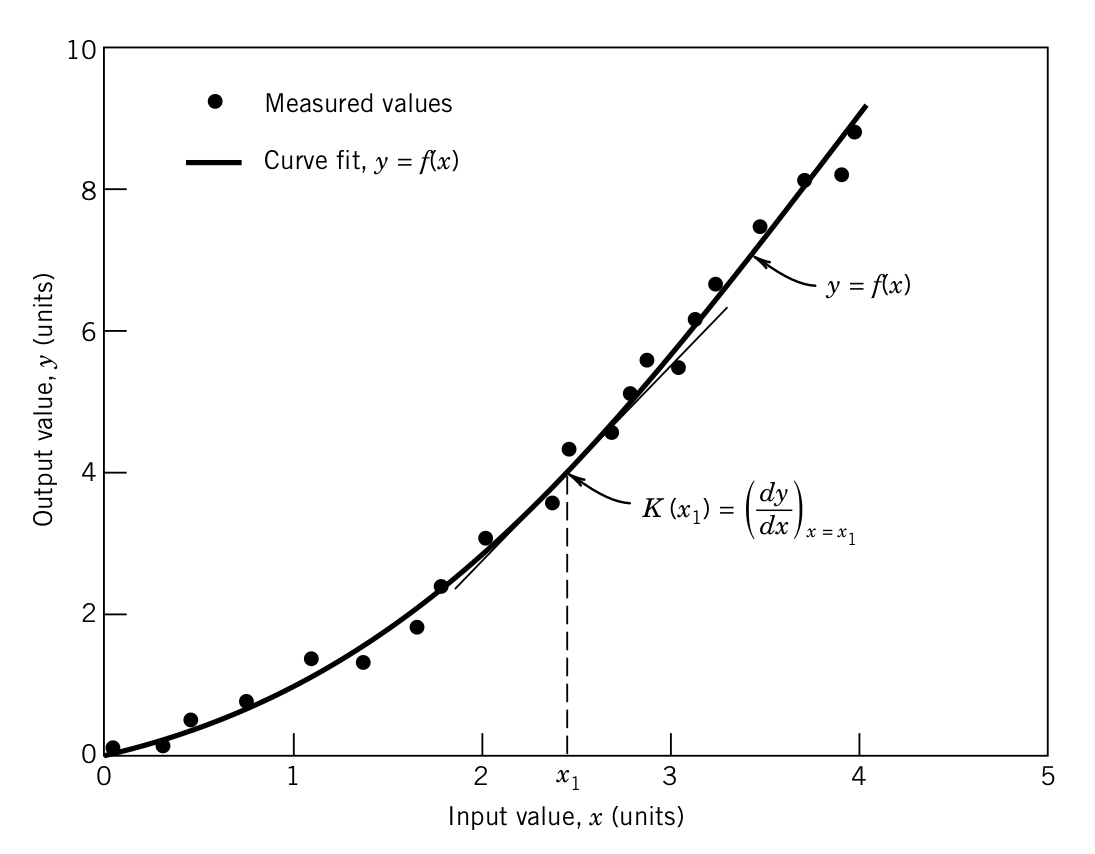
\includegraphics[scale=.14]{images/calibration_curve.png} 

				\small
				Assume $R=120\Omega$ for all resistors and the bridge is balanced in a condition of zero strain. What is the {\PN static sensitivity} of the gauge and bridge circuit described? \vspc

				\scalebox{1}{K=}\vspc

				\end{multicols}

				{\tiny Text. Images: Theory and Design for Mechanical Measurements}

			\end{frame}

			\begin{frame}
				\frametitle{\sectionIIsubsectionIVtitle}


			\end{frame}
		
	% Section III
	\section{\sectionIIItitle}\label{sectionIII}

		% section III Outline
		\begin{frame}
			\large \textbf{Topic 3 - \sectionIIItitle} \vspace{3mm}\\

			\begin{itemize}
				\item \hyperlink{sectionIIIsubsectionI}{\sectionIIIsubsectionItitle} \vspc %  section III subsection I
				\item \hyperlink{sectionIIIsubsectionII}{\sectionIIIsubsectionIItitle} \vspc % section III subsection II
				\item \hyperlink{sectionIIIsubsectionIII}{\sectionIIIsubsectionIIItitle} \vspc % section III subsection III
				\item \hyperlink{sectionIIIsubsectionIV}{\sectionIIIsubsectionIVtitle} \vspc % section III subsection IV
			\end{itemize}

		\end{frame}

		% section III subsection I
		\subsection{\sectionIIIsubsectionItitle}\label{sectionIIIsubsectionI}

			\begin{frame}
				\frametitle{\sectionIIIsubsectionItitle}

				\bigskip

				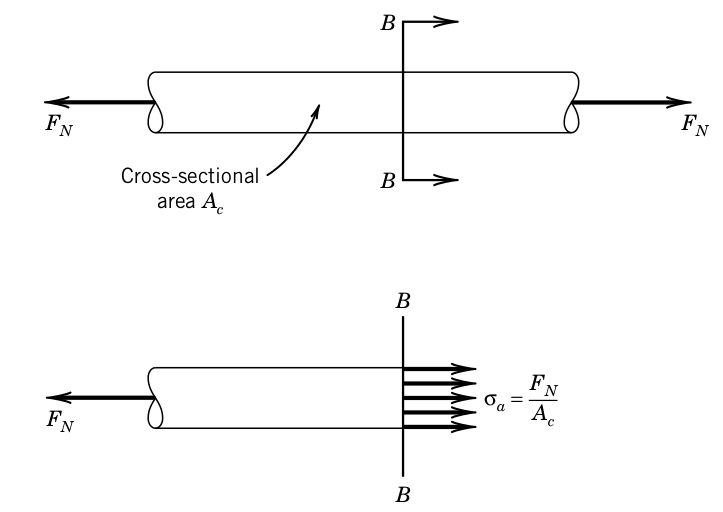
\includegraphics[scale=.25]{images/strain_fig1.png}
			
				\btVFill
			

			\end{frame}

			\begin{frame}
				\frametitle{\sectionIIIsubsectionItitle}
		
			\end{frame}

		% section III subsection II
		\subsection{\sectionIIIsubsectionIItitle}\label{sectionIIIsubsectionII}	

			\begin{frame}
				\frametitle{\sectionIIIsubsectionIItitle}

				\bigskip

				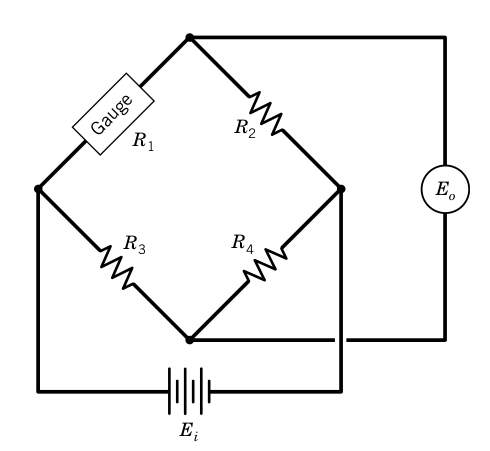
\includegraphics[scale=.2]{images/gauge_in_bridge_quarter.png} 
				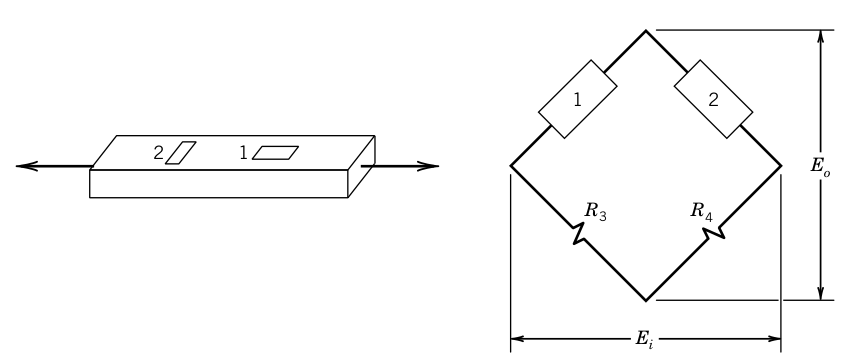
\includegraphics[scale=.2]{images/gauge_in_bridge_half.png} 
				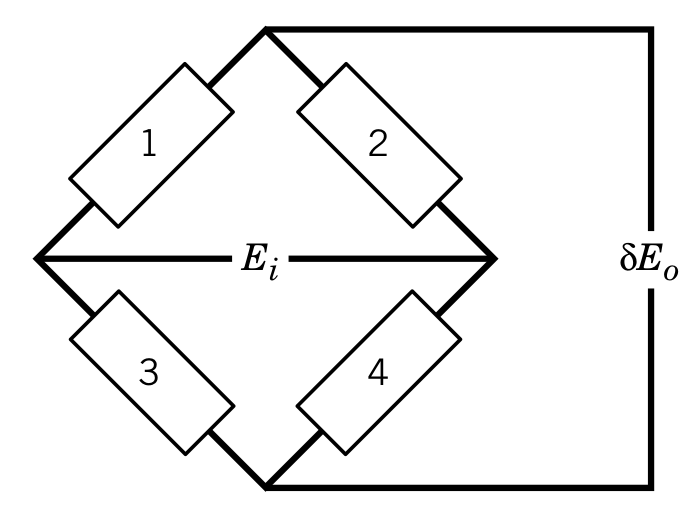
\includegraphics[scale=.16]{images/gauge_in_bridge_full.png}

				\btVFill

			\end{frame}

			\begin{frame}
				\frametitle{\sectionIIIsubsectionIItitle}

				\bigskip
				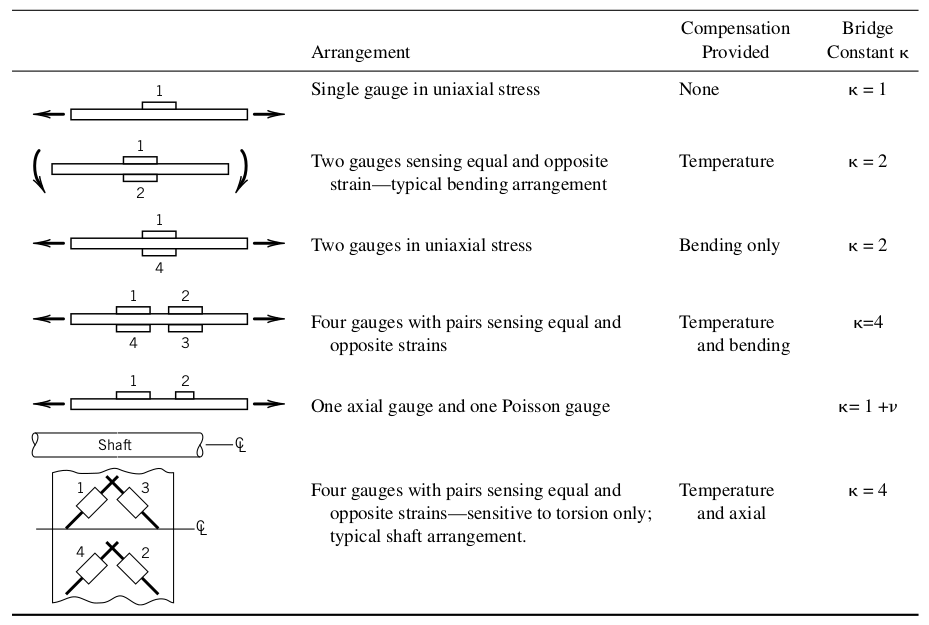
\includegraphics[scale=.3]{images/gauge_configurations.png}
			
				\btVFill

			\end{frame}

			\begin{frame}
				\frametitle{\sectionIIIsubsectionIIItitle}

				\bigskip
				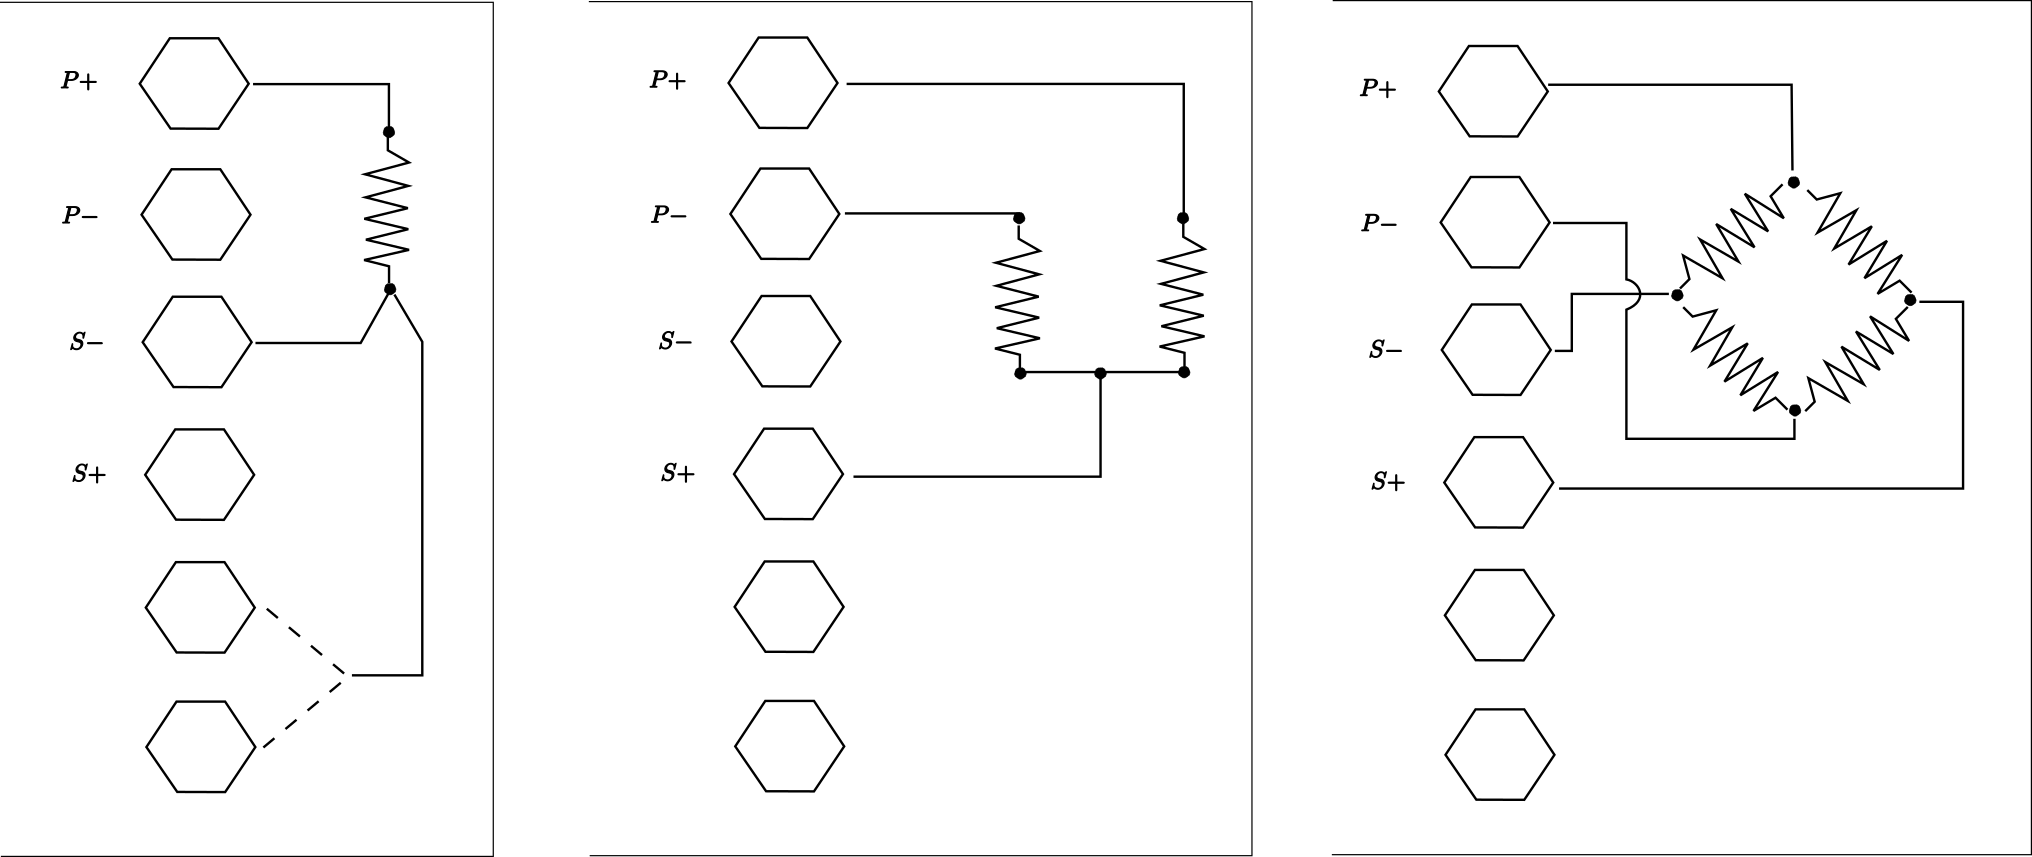
\includegraphics[scale=.22]{images/quarter_half_full.png}

				\btVFill
				
			\end{frame}

			\begin{frame}
				\frametitle{\sectionIIIsubsectionIIItitle}



			\end{frame}

		% section III subsection III
		\subsection{\sectionIIIsubsectionIIItitle}\label{sectionIIIsubsectionIII}	

			\begin{frame}[containsverbatim]
				\frametitle{\sectionIIIsubsectionIIItitle}\scriptsize


				\begin{itemize}

					\item The instructions are on the unit. 

					\item The balancing process is completed after changing any wiring. 

				\end{itemize}

				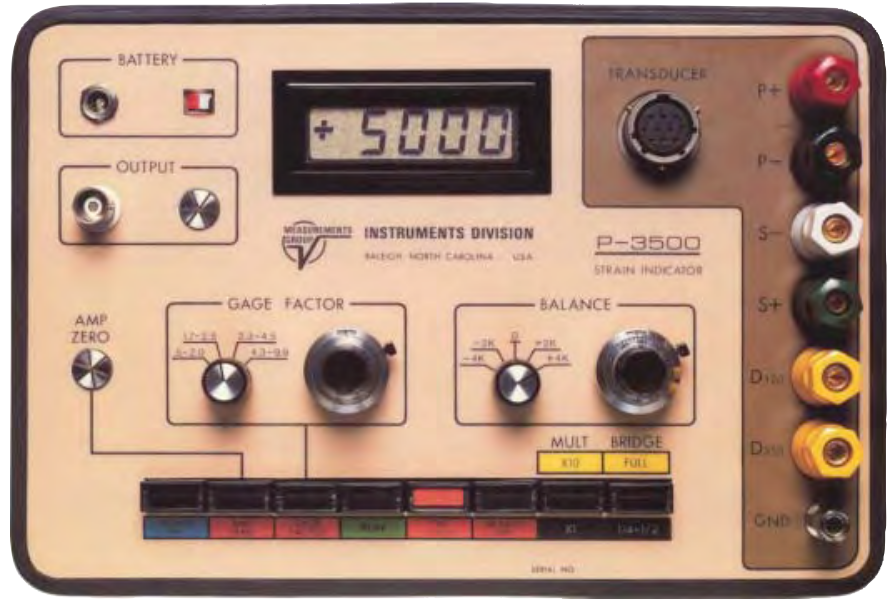
\includegraphics[scale=.228]{images/p3500_fig1.png}

			\end{frame}

			\begin{frame}[containsverbatim]
				\frametitle{\sectionIIIsubsectionIIItitle}\scriptsize
			

			
			\end{frame}

		% section III subsection IV
		\subsection{\sectionIIIsubsectionIVtitle}\label{sectionIIIsubsectionIV}	
		
		% section III subsection IV - Frame I
		\begin{frame} \scriptsize
		\frametitle{\sectionIIIsubsectionIVtitle}
		\bigskip


			\begin{itemize}

			\item The P3500/P3 is expensive, but it is a reliable instument. The ME department has used them for years with success. \vspc

			\item The manufacturer {\it Vishay Group} has a {\it more} modern solution with DAQ and multiple channels. \vspc

			\item There are a variety of low cost alternative options available.

			\begin{itemize}
			\item \href{https://learn.sparkfun.com/tutorials/getting-started-with-load-cells/strain-gauge-basics}{Sparkfun - strain gauge basics}
			\item \href{https://www.robotshop.com/en/strain-gauge-load-cell-amplifier-shield-2ch.html}{Robot Shop}

			\item \href{https://www.elecrow.com/strain-gauge-module-p-735.html}{elecrow}
			\end{itemize}

			\end{itemize}


		\btVFill

		\end{frame}
	

\end{document}





